\documentclass{article}
\usepackage{tikz, bm}
\newcommand{\vv}[1]{\bm{#1}}
\begin{document}
\begin{center}
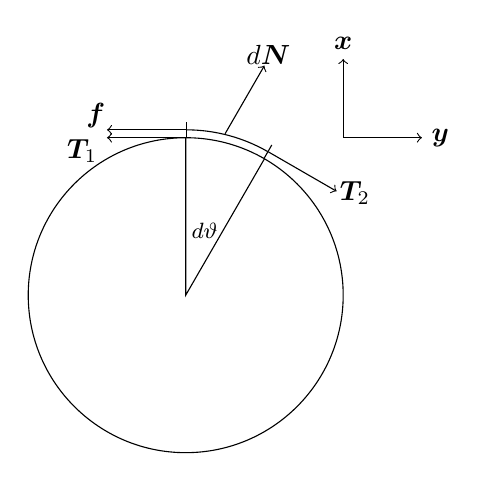
\begin{tikzpicture}
\draw (0,0) circle [radius=2];
\draw (0,2) -- (0,0) -- (1,1.732);
\draw [|-|](0,2.1) arc [start angle = 90, end angle = 60, radius = 2.1];
\draw [->] (0,2) -- (-1,2);
\draw [rotate around={-30:(1.05,1.82)}][->] (1.05,1.82) -- (2.05,1.82);
\draw [rotate around={-30:(0.5,2.05)}][->] (0.5,2.05) -- (0.5, 3.05);
\draw [->] (0,2.1) -- (-1,2.1);
\node [above right] at (-0.05,0.6) {\footnotesize{\(d\vartheta\)}};
\node at (1.05,3.05) {\(d\vv N\)};
\node at (2.15,1.3) {\(\vv T_2\)};
\node [below left] at (-1,2.1) {\(\vv T_1\)};
\node [above left] at (-0.9,2) {\(\vv f\)};
\draw [<->] (2,3) -- (2,2) -- (3,2);
\node [above] at (2,3) {\(\vv x\)};
\node [right] at (3,2) {\(\vv y\)};
\end{tikzpicture}
\end{center}
\end{document}